\chapter{Результаты и анализ}
\label{sec:Chapter5} \index{Chapter5}

В главе собраны количественные и качественные результаты разработанных моделей, а также выделены затрачиваемые ресурсы при инференсе сетей.
Сначала оценивается вклад отдельных компонентов (обратный ablation семейства
LLW-Former \ref{sec:ablation}), затем разбираются отвергнутые
альтернативы \ref{sec:negative} и проверка высокочастотного дискриминатора HF-D \ref{sec:hfd}.
Завершает главу сопоставление с опубликованными
методами трансляции SAR\,$\to$\,optical на датасете SEN1-2.

% ======================================================================
\section{Условия экспериментов}
\label{sec:setup}

Все версии семейства LLW-Former обучались на одном и том же подмножестве датасета
SEN1-2: пять репрезентативных сцен (5, 45, 52, 84 и 100), что после очистки даёт
11\,315 парных изображений. Разрешение тренировочных и валидационных пар
$256\times 256$ пикселей. Оптимизатор AdamW, базовый learning
rate $2{\cdot}10^{-4}$ как для генератора, так и для дискриминатора,
$\beta_{1}=0.5$, $\beta_{2}=0.999$. Расписание learning rate константа на
первых 150~эпохах и линейный спад на последних~50. Точность BF16-mixed, которая позволяет ускорить обучения без существенных потерь в качестве.
Для финальной версии дополнительно применено предварительное выравнивание пар в
градиентной области.

\section{Протокол валидации}
Все модели обучались на одних и тех же пяти сценах,
поэтому основной валидацией служит разбиение по этим же сценам с сохранением классового представление.
Числа в таблицах~\ref{tab:ablation} и~\ref{tab:sota} приведены по нему и соответствуют
лучшему чекпоинту (эпоха максимума PSNR), а не покомпонентному максимуму по эпохам.
Контролируемая проверка HF-D (таблица~\ref{tab:hfd_final}) выполнена отдельно. На
полном валидационном наборе SEN1-2 (2263 пары). Абсолютные
значения по двум протоколам напрямую несопоставимы, и сравнение HF-D проводится
строго внутри одного протокола.

Публикуемые работы по SEN1-2 (Pix2Pix, CycleGAN, диффузионные подходы) также обучаются
не на полном датасете ($\approx 282$~тыс. пар), а на подмножествах в диапазоне
1,6--12,8~тыс. пар. Использованное подмножество (11,3~тыс. пар, 5~сцен) приходится
на середину этого диапазона, поэтому сравнение с опубликованными метриками корректно.
Качественное сравнение почти наверняка не представляется возможным, так как подвыборки разные.
Основное сравнение нацелено на предыдущие методы, в частности CFRWD GAN. Потому были выбраны идентичные подвыборки.

% ======================================================================
\section{Обратный ablation семейства LLW-Former}
\label{sec:ablation}

Таблица~\ref{tab:ablation} приводит результаты последовательнх абляций: от
финальной модели шаг за шагом убираются архитектурные и регуляризационные
компоненты вплоть до базовой версии. Каждая строка отличается от предыдущей
удалением ровно одной компоненты при прочих фиксированных настройках.

\begin{table}[H]
  \caption{Обратный ablation семейства LLW-Former: строки читаются сверху вниз, от
           финальной конфигурации к базовой, каждый шаг убирает группу
           компонентов (= откат на версию назад). Метрики~--- лучшие по
           валидации (на эпохе максимума PSNR), 5-сценовый валидационный сплит
           SEN1-2. Стрелки указывают направление улучшения}
  \label{tab:ablation}
  \centering
  \small
  \begin{tabular}{p{0.40\linewidth}cccc}
    \toprule
    Конфигурация & PSNR, дБ\,$\uparrow$ & SSIM\,$\uparrow$ & FID\,$\downarrow$ & LPIPS\,$\downarrow$ \\
    \midrule
    LLW-Former Base \textbf{(финальная)}              & \textbf{18.54} & \textbf{0.432} & \textbf{58.50} & \textbf{0.241} \\
    \;\;$-$ ёмкость бэкбона: Base $\to$ Tiny           & 17.28 & 0.369 & 73.00 & 0.311 \\
    \;\;$-$ выравнивание пар (Tiny без alignment)      & 17.06 & 0.348 & 84.00 & 0.314 \\
    \;\;$-$ перцептивные потери (MS-SSIM/LPIPS/FFL/NCE)& 14.85 & 0.297 & 91.50 & 0.422 \\
    \;\;$-$ покомпонентная Хаар-потеря (только IHaar)  & 13.02 & 0.273 & 87.50 & 0.438 \\
    \;\;$-$ обратное Хаар-преобр.\ (RGB-голова, v0.3)  & 12.91 & 0.265 & 73.50 & 0.436 \\
    \bottomrule
  \end{tabular}
\end{table}

\subsection{Интерпретация результатов ablation}

Снижение ёмкости бэкбона (Base~$\to$~Tiny) стоит модели 1.26~дБ PSNR и 0.063~SSIM,
ухудшает FID с 58.5 до 73.0 ($+25\%$), а LPIPS~--- с 0.241 до 0.311. Перцептивные
метрики масштабируются с ёмкостью модели лучше пиксельных, и конфигурация Base
остаётся лучшей по всем четырём метрикам.

Отказ от предварительного выравнивания пар (тот же Tiny на сырых данных) почти не
трогает PSNR (17.28~$\to$~17.06), но заметно ухудшает FID (73.0~$\to$~84.0). Причина
разобрана в разделе~\ref{sec:negative}. Кратко разрегистрация бьёт по перцептивному
качеству сильнее, чем по пиксельному.

Дальнейшее удаление перцептивных компонентов функции потерь (MS-SSIM, LPIPS, FFL,
PatchNCE) даёт наибольшее ухудшение. PSNR падает до 14.85, SSIM до 0.297, FID
растёт до 91.5, LPIPS до 0.422. Перцептивная и контрастная регуляризация снимают
«потолок», характерный для парных GAN на разрегистрированных датасетах.

Если оставить только обратное Хаар-преобразование, сняв покомпонентную Хаар-потерю,
метрики откатываются к уровню $\approx 13$~дБ. Согласованность выходной головы с
базисом сама по себе не переходит в показатели без специально подобранной потери.
Замена Хаар-головы на классическую RGB-голову (версия v0.3) даёт нижнюю границу
12.91~дБ. Каждое решение вносит независимый вклад, а наибольшее влияние на качество
оказывают перцептивная регуляризация и ёмкость бэкбона.

\begin{figure}[!ht]
  \centering
  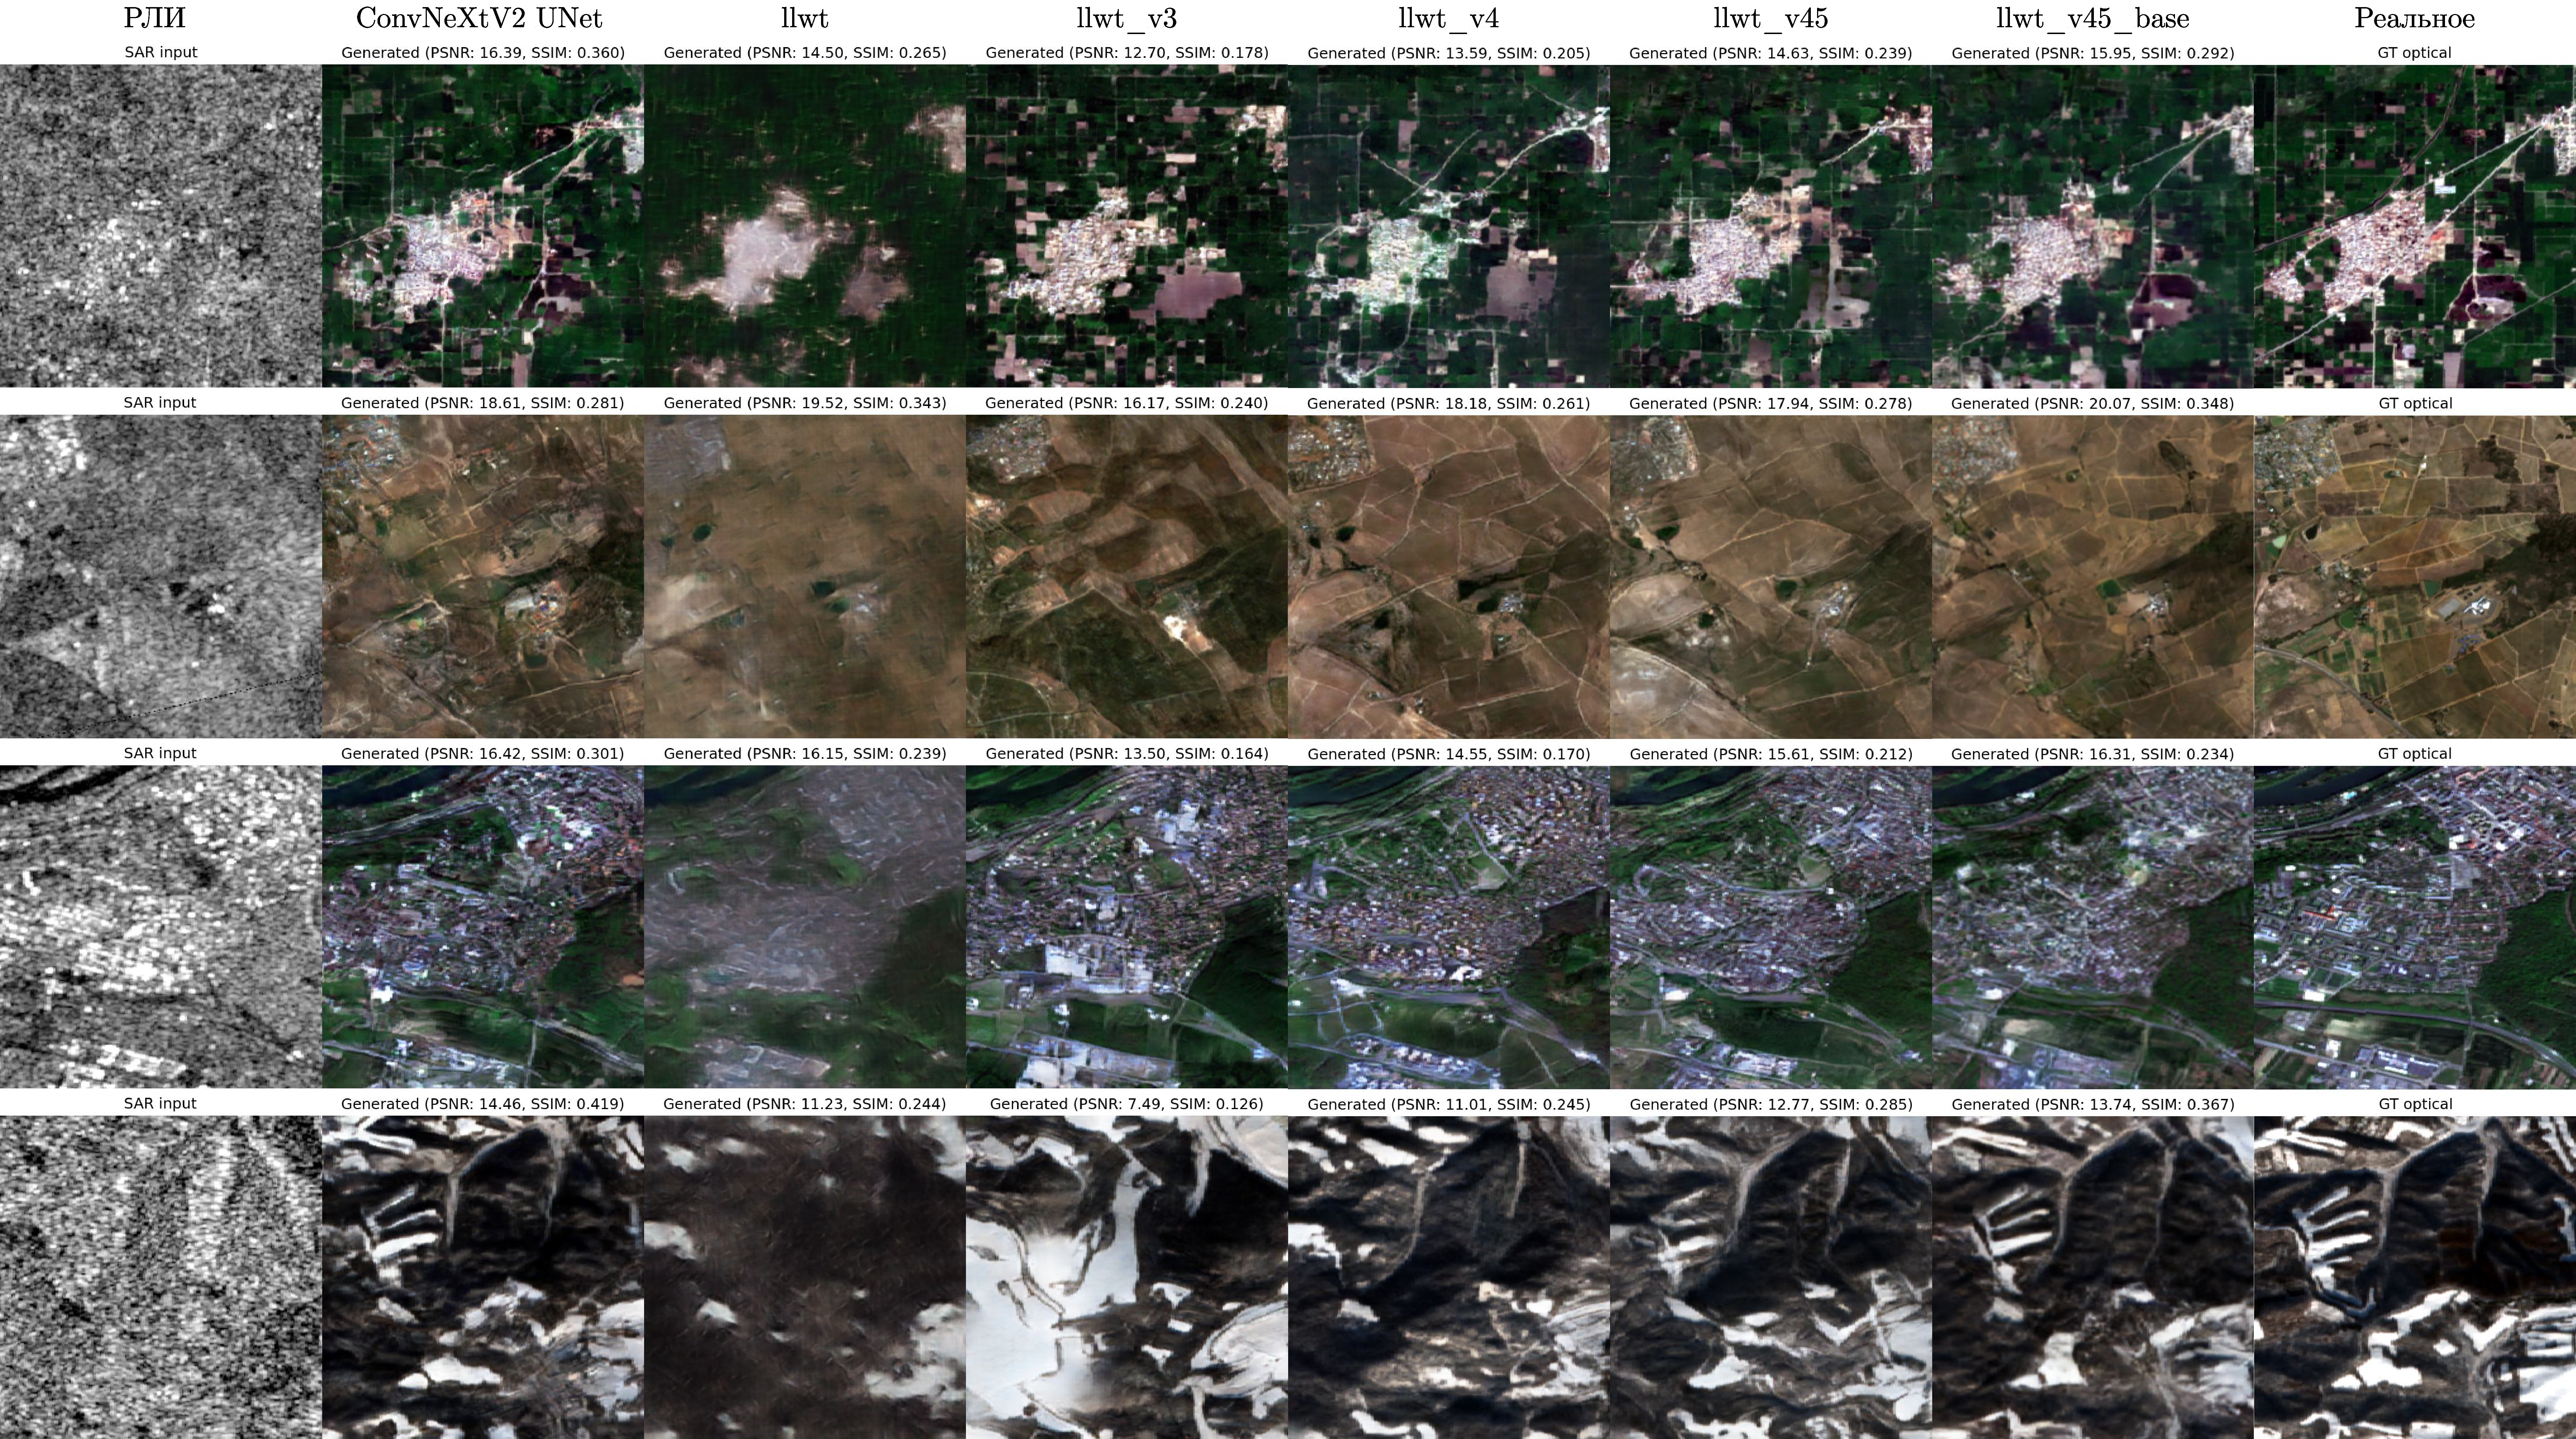
\includegraphics[width=\linewidth]{./images/llwt/output/llwt_comparison.pdf}
  \caption{Качественное сравнение моделей на репрезентативных парах валидационной
           выборки SEN1-2. Колонки слева направо: SAR-вход; базовая модель
           ConvNeXt~V2\,+\,U-Net; последовательные версии семейства
           (llwt, llwt\_v3, llwt\_v4, llwt\_v45) и конфигурация llwt\_v45\_base;
           эталонное оптическое изображение. Под каждой реконструкцией указаны
           PSNR/SSIM соответствующей пары}
  \label{fig:abl_qual}
\end{figure}

\begin{figure}[!ht]
  \centering
  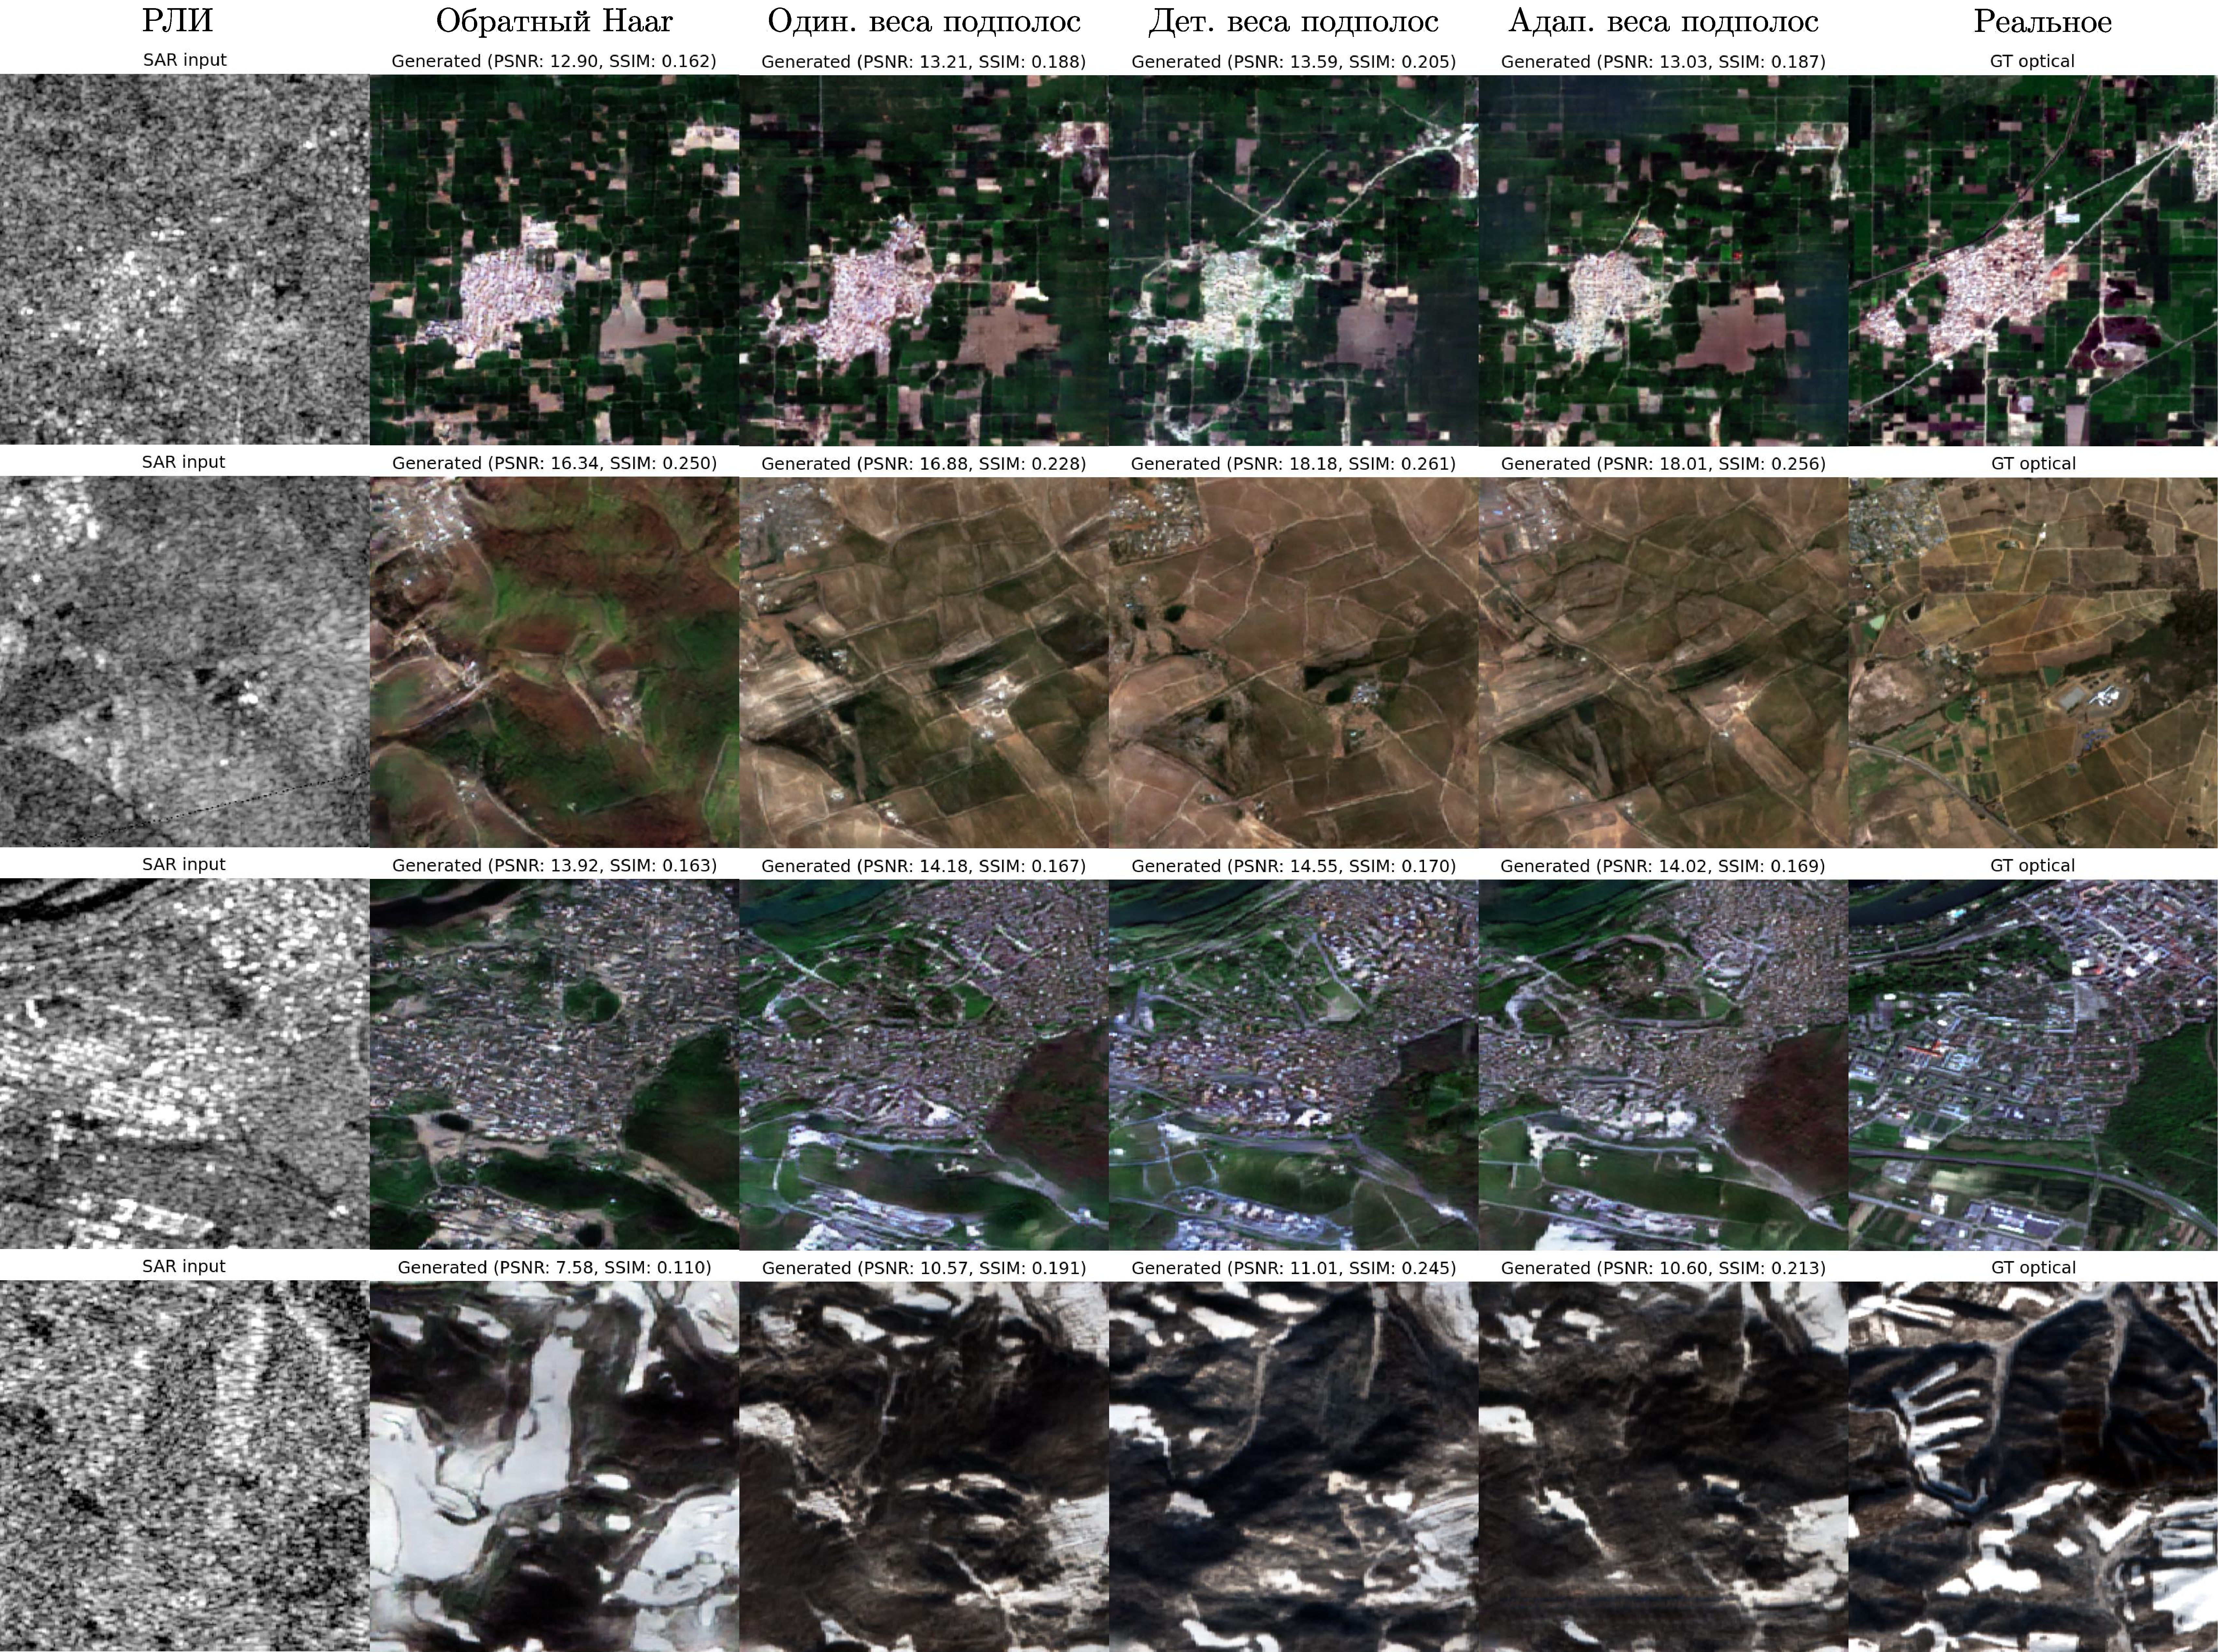
\includegraphics[width=\linewidth]{./images/llwt/output/llwt_ablation.pdf}
  \caption{Абляция стратегии взвешивания поддиапазонов Хаара (на базе llwt\_v4).
           Колонки: SAR-вход; только обратное Хаар-преобразование без покомпонентной
           потери; равные веса поддиапазонов; усиленные веса детальных поддиапазонов
           (LH/HL/HH); адаптивные (обучаемые) веса; эталон. По перцептивным метрикам
           (FID/LPIPS) лучшим оказывается усиление детальных поддиапазонов, по
           PSNR~--- равные веса, по SSIM~--- адаптивные; для итоговой модели выбраны
           детальные веса как наиболее благоприятные для резкости}
  \label{fig:abl_subband}
\end{figure}

% ======================================================================
\section{Диагностика узкого места и отвергнутые альтернативы}
\label{sec:negative}

Чтобы установить источник остаточного размытия, обученную финальную модель
прогнали на отложенном наборе выровненных валидационных патчей и разложили её ошибку
двумя способами: по пространственной частоте и по поддиапазонам Хаар-разложения
(таблица~\ref{tab:errorprofile}).

\begin{table}[H]
  \centering
  \caption{Профиль ошибки базовой версии генератора на отложенных выровненных
           патчах. Относительная ошибка поддиапазона~--- покомпонентная $L_{1}$,
           нормированная на энергию поддиапазона; отношение радиальной мощности~---
           $P_{\text{fake}}/P_{\text{opt}}$ в октаве частот (цель $=1.0$)}
  \label{tab:errorprofile}
  \begin{tabular}{lcc}
    \toprule
    Величина & Значение & Интерпретация \\
    \midrule
    Ошибка яркость / цветность      & $9.43$ / $4.5$ & цвет \emph{не} узкое место \\
    Глобальный сдвиг цвета          & $-0.003$ & нет цветового сдвига \\
    Отн. ошибка LL (низкие частоты) & $0.33$ & крупная структура восстановлена \\
    Отн. ошибка деталей (LH,HL,HH)  & $\geq 1.3$ & детали фазово-декоррелированы \\
    Отношение деталь / LL           & $4.2$ & детали в $4\times$ хуже LL \\
    Отношение мощности (средние частоты) & $0.66$ & \textbf{размытие} \\
    Отношение мощности (высокие частоты) & $1.14$ & некогерентный шум \\
    \bottomrule
  \end{tabular}
\end{table}

Профиль указывает на структурный дефицит, а не на цветовой. Низкочастотный
поддиапазон LL восстановлен хорошо (относительная ошибка $0.33$), тогда как
детальные поддиапазоны фазово-декоррелированы: их относительная ошибка превышает
единицу. Средние частоты модель недопроизводит (мощность $0.66$, типичная
сигнатура размытия), а высокие, наоборот, перепроизводит в виде некогерентного
шума ($1.14$). Тяжелее всего приходится низкотекстурным водным сценам. В них одному
входу SAR отвечает множество правдоподобных оптических изображений.

К структурному дефициту добавляется геометрия. Жёсткое попарное выравнивание показывает медианный сдвиг в $1.23$~пикселя.
У $58\%$ пар он превышает один пиксель, у $31\%$ два пикселя, а 90-й перцентиль доходит
до $5.3$~пикселя. При таком разбросе позиционно-точная супервизия высоких частот
заведомо ненадёжна.

До выбора итогового решения были проверены две напрашивающиеся гипотезы. Обе
пришлось отвергнуть, и оба отрицательных результата мотивируют выбор HF-D.

\subsection{Негативный результат 1: плотная обучаемая регистрация неосуществима}

Самый прямой ответ на разрегистрацию это обучить плотное поле деформации $\phi$,
которое подгоняет эталон под геометрию генератора до вычисления пиксельных потерь.
Поле $\phi$ оценивалось из спекл-устойчивого поддиапазона LL, но выравниватель
оказался инертным. За 130~эпох величина $|\phi|$ так и осталась на уровне
$\sim 0.07$~пикселя, то есть на уровне шума дискретизации bf16. Переход на точность fp32
ничего не изменил.

Причину выявили несколько контролируемых проб. Даже с отключённым регуляризатором
и замороженным генератором градиент фиделити доводил $\phi$ только до
$\sim 0.2$~пикселя, что заметно ниже измеренного сдвига в $1.23$~пикселя. Дело
в разрыве между модальностями. При прямом измерении локального сходства SAR и оптики
(нормированная кросс-корреляция градиентов, $\mathrm{NCC}$) оно оказывается почти
нулевым: $\mathrm{NCC}\approx 0.02$. Сам сдвиг при этом реален и уверенно ловится
глобально, жёсткой фазовой корреляцией, тогда как плотного локального сигнала
сходства, на который мог бы опереться обучаемый выравниватель, нет. Это подтвердила
и прямая проба: локальный NCC-объектив выдавал градиент, но собственную потерю не
уменьшал.
\textbf{Вывод}: плотная неконтролируемая регистрация SAR\,$\to$\,optical не обучается
из сходства изображений. Разрегистрацию нужно обрабатывать устойчивым к сдвигу
сигналом супервизии, а не пытаться её скорректировать.

\subsection{Негативный результат 2: статистические потери ранжируют резкость, но не синтезируют её}

Если сдвиг нельзя исправить, детали можно восстанавливать потерей, которой этот
сдвиг безразличен. Была проверена sliced-Wasserstein-потеря (SWD) на детальных
поддиапазонах Хаара. Она сопоставляет не пиксели, а отсортированные распределения
коэффициентов, поэтому нечувствительна и к перестановке, и к сдвигу.

Как критерий оценки SWD ведёт себя ожидаемо. При синтетическом сдвиге в
$1.5$~пикселя пиксельная $L_{1}$-потеря на деталях предпочитает размытое
предсказание резкому, но сдвинутому ($0.037 < 0.056$), тогда как SWD предпочитает
резкое ($0.0095 < 0.025$, запас в $2.6$~раза) и почти не реагирует на сам сдвиг
(индекс чувствительности $0.13$). Этим и объясняется природа размытия. При
разрегистрированном эталоне пиксельные потери вознаграждают размытый выход.

Тем не менее отложенный A/B-тест (раздел~\ref{sec:hfd}) забраковал SWD
в роли двигателя обучения. При замене детальной $L_{1}$ на детальную SWD выход стал
не резче, а чуть мягче: мощность средних частот $0.629$ против $0.652$, мощность
деталей $0.582$ против $0.626$, LPIPS $0.311$ против $0.307$.
\textbf{Вывод}: Потеря,
которая лишь ранжирует резкий выход выше размытого, своей минимизацией резкого выхода
не создаёт. Сопоставление гистограмм коэффициентов задаёт энергетический бюджет
(сколько деталей должно быть в сумме), но не указывает, куда именно поставить край,
то есть не даёт пространственного градиента для когерентной структуры. Отсюда и
решение: когерентную высокочастотную структуру способен сформировать только
состязательный сигнал. Позиционно-выровненная пиксельная супервизия дала бы тот же
эффект, но в наших условиях она недоступна.

% ======================================================================
\section{Высокочастотный дискриминатор: верификация}
\label{sec:hfd}

\subsection{Протокол}

Целевой эффект~--- явление обобщения. Размытие от разрегистрации проявляется
лишь когда модель не может запомнить сдвиг каждой пары. Переобучение на одном
батче здесь не является корректной проверкой, поскольку способствует пиксельному $L_{1}$ за счёт
запоминания, поэтому оценка ведётся на отложенной выборке A/B. Из общей
инициализации два плеча, идентичные во всём кроме проверяемой переменной,
обучаются 2200 шагов генератора на сырых (невыровненных) данных SEN1-2, а
измеряются на фиксированном отложенном множестве из 32 пар, которые модель не видела при
обучении. Резкость считывается по радиальному отношению мощности средних частот
(цель $1.0$). Когерентность~--- по отношению мощности высоких частот ($\gg 1.15$
означает некогерентный шум), а перцептивное качество по LPIPS. PSNR/SSIM
приводятся, но, как было выявлено в \ref{sec:Chapter4}, не являются достаточным доказательством отсутствия размытости изображения.
Наоборот, при разрегистрированном эталоне они вознаграждают размытие.

\subsection{Результаты отложенного A/B}

Таблица~\ref{tab:hfd_ab} приводит отложенный A/B. Плечо HF-D повышает отношение
мощности средних частот на каждой контрольной точке и поднимает энергию деталей к
цели. Отношение высоких частот возрастает с $0.643$ до $0.696$, оставаясь
значительно ниже порога шума $1.15$. LPIPS не меняется, дискриминатор устойчив всё
обучение ($d$-loss $0.23\!\to\!0.25$, без расходимости). Тот же стенд отверг
статистическую (SWD) потерю, сдвинувшую метрики в неверную сторону.

\begin{table}[H]
  \centering
  \caption{Отложенный A/B-тест обобщения после 2200 шагов на сырых
           (разрегистрированных) SEN1-2. Отношения мощности средних частот и деталей
           целятся в $1.0$ (выше $=$ резче); отношение высоких частот должно
           приближаться к $1.0$ снизу ($\gg 1.15$~--- некогерентный шум).
           Baseline~--- полный набор потерь; HF-D~--- baseline $+\,\lambda_H
           \mathcal{L}^G_H$; отвергнутое плечо SWD показано для контраста}
  \label{tab:hfd_ab}
  \begin{tabular}{lccc}
    \toprule
    Метрика (отложенная) & Baseline & \textbf{HF-D} & SWD (отвергнут) \\
    \midrule
    Отношение мощности средних частот $\uparrow$ & $0.652$ & $\mathbf{0.695}$ & $0.629$ \\
    Отношение мощности деталей $\uparrow$         & $0.626$ & $\mathbf{0.687}$ & $0.582$ \\
    Отношение мощности высоких частот ($\to 1.0$) & $0.643$ & $0.696$      & --- \\
    LPIPS $\downarrow$                   & $0.307$ & $0.307$          & $0.311$ \\
    PSNR (не судья резкости)             & $17.08$ & $16.98$          & $17.14$ \\
    SSIM                                 & $0.298$ & $0.294$          & $0.300$ \\
    \bottomrule
  \end{tabular}
\end{table}

\subsection{Контролируемое сравнение на полной валидации}

A/B на 2200 шагах устанавливает знак и когерентность эффекта, но не его
насыщенную величину. Для итоговой оценки финальная модель с HF-D и её базовый аналог
($\lambda_H=0$) прогнаны на полном валидационном сплите (2263 пары) через
одни и те же выборки и оба EMA-генератора (таблица~\ref{tab:hfd_final}). HF-D
снижает LPIPS на $8.8\%$ (0,330~$\to$~0,301) и FID примерно на $11\%$
($\approx 84 \to 75$) при практически неизменных пиксельных метриках
($-0.01$~дБ PSNR, $-0.005$~SSIM).

\begin{table}[H]
  \centering
  \caption{Финальная модель с HF-D ($\lambda_H{=}1$) против базового аналога
           ($\lambda_H{=}0$) на полном валидационном сплите (2263 пары, одни и те же
           выборки, оба EMA-генератора). PSNR/SSIM/LPIPS вычислены контролируемым
           скриптом на идентичных выборках; FID измерен отдельно по полному прогону
           (отсюда $\approx$)}
  \label{tab:hfd_final}
  \begin{tabular}{lcccc}
    \toprule
    Модель & PSNR\,$\uparrow$ & SSIM\,$\uparrow$ & LPIPS\,$\downarrow$ & FID\,$\downarrow$ \\
    \midrule
    Базовая ($\lambda_H{=}0$)        & $18.50$ & $0.352$ & $0.330$ & $\approx 84$ \\
    \textbf{HF-D} ($\lambda_H{=}1$)  & $18.49$ & $0.347$ & $\mathbf{0.301}$ & $\mathbf{\approx 75}$ \\
    \bottomrule
  \end{tabular}
\end{table}

\begin{figure}[!ht]
  \centering
  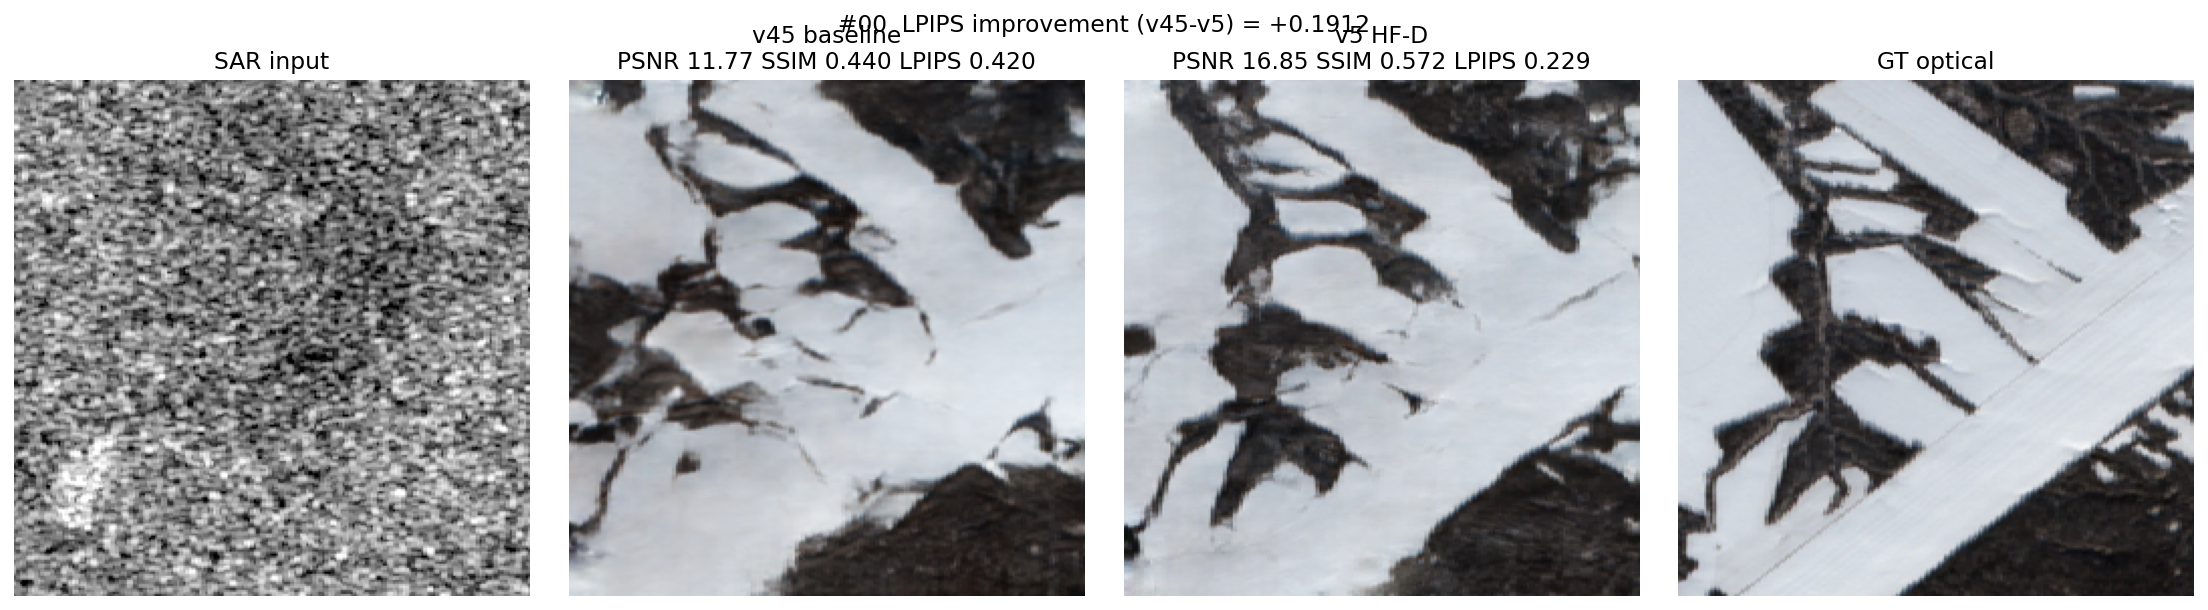
\includegraphics[width=\linewidth]{./images/llwt/output/cmp_00_sample1542_dLPIPS0.191.png}\\[4pt]
  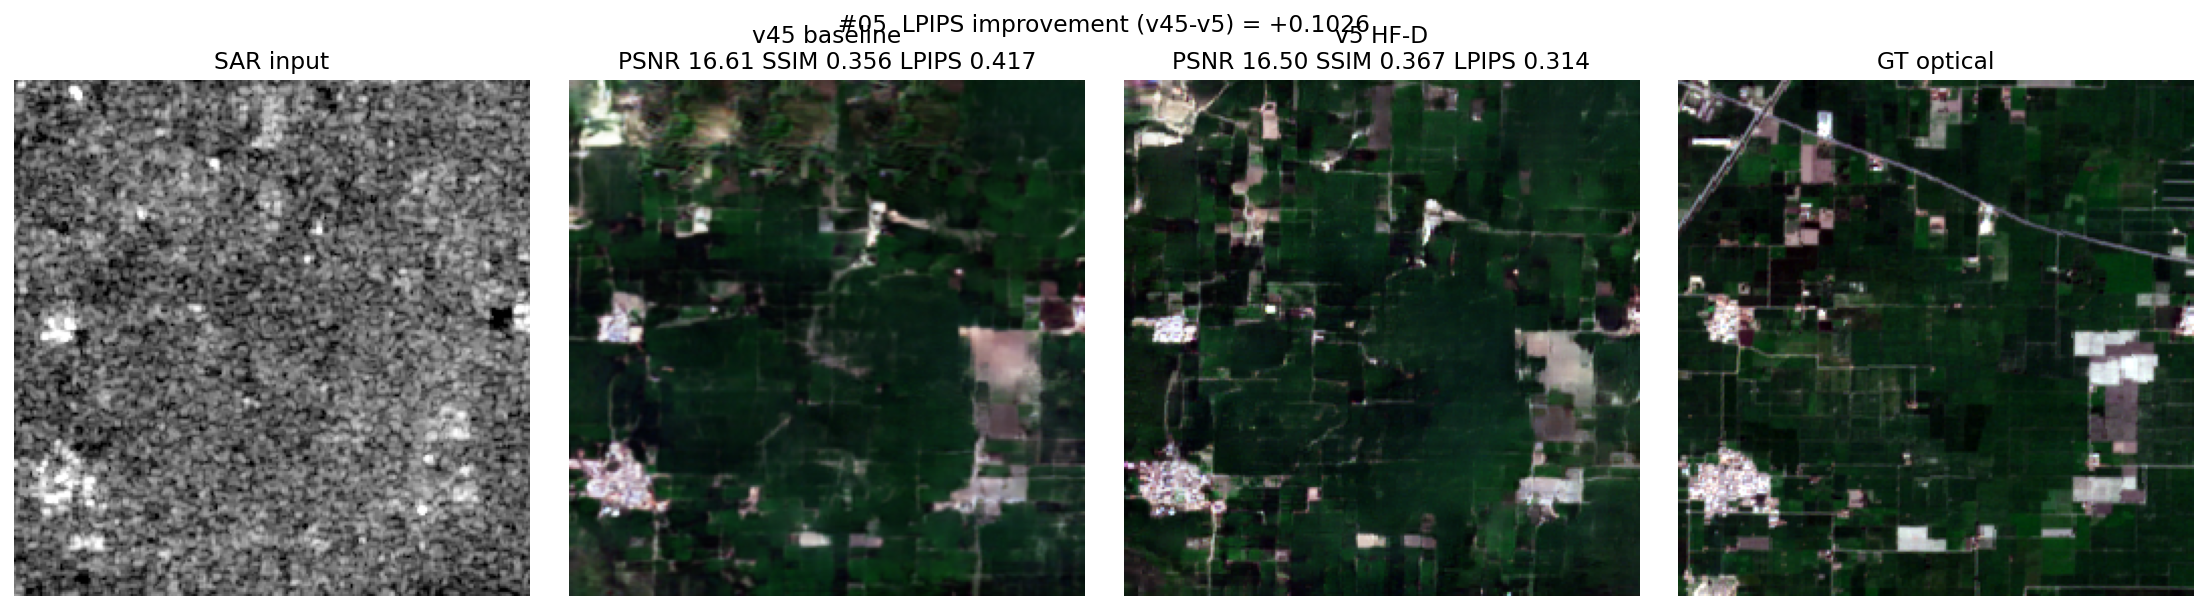
\includegraphics[width=\linewidth]{./images/llwt/output/cmp_05_sample0874_dLPIPS0.103.png}
  \caption{Контролируемое качественное сравнение базовой модели ($\lambda_H{=}0$) и
           модели с HF-D ($\lambda_H{=}1$) на отложенных парах (одинаковый вход, оба
           EMA-генератора). Колонки: SAR-вход; базовая; HF-D; эталон; под каждой
           реконструкцией~--- PSNR/SSIM/LPIPS. HF-D формирует чёткие границы и
           когерентную высокочастотную структуру, совпадающую с эталоном, без шумовых
           артефактов: например, на верхней паре LPIPS улучшается с 0.420 до 0.229
           (а PSNR~--- с 11.77 до 16.85), на нижней~--- с заметным приростом резкости. Дополнительные изображения можно увидеть в \ref{sec:Appendix}.}
  \label{fig:hfd_qual}
\end{figure}

% ======================================================================
\section{Сравнение с существующими методами}
\label{sec:results:sota}

Таблица~\ref{tab:sota} сопоставляет финальные конфигурации LLW-Former с
опубликованными методами трансляции SAR\,$\to$\,optical на SEN1-2. Данные сторонних
методов взяты из соответствующих публикаций, приведённые диапазоны учитывают различия
в подвыборках и протоколах оценки.

\begin{table}[H]
  \caption{Сравнение LLW-Former с существующими методами SAR\,$\to$\,optical на SEN1-2}
  \label{tab:sota}
  \centering
  \small
  \begin{tabular}{lcccc}
    \toprule
    Метод & PSNR, дБ\,$\uparrow$ & SSIM\,$\uparrow$ & LPIPS\,$\downarrow$ & FID\,$\downarrow$ \\
    \midrule
    Pix2Pix                   & 12.79 & 0.1793 & 0.4834 & 113.87 \\
    CycleGAN                 & 11.54 & 0.1717 & 0.4974 & 89.38  \\
    MUNIT                     & 14.1--15.0 & 0.22--0.26 & 0.40--0.47 & 165--220 \\
    INRECGAN                & 15.74 & 0.2934 & 0.4613 & 73.96  \\
    DTGAN                        & 13.52 & 0.1939 & 0.5266 & 82.41  \\
    ScE-GAN                     & 11.04 & 0.1721 & 0.5173 & 78.94  \\
    EdgeGAN / TerrainGAN  & 15.4--17.2 & 0.27--0.32 & 0.34--0.41 & 130--180 \\
    DDA-GAN                    & 11.69 & 0.1743 & 0.4990 & 87.14  \\
    CFRWD-GAN                    & 17.2--18.3 & 0.29--0.35 & 0.31--0.37 & 116--150 \\
    \midrule
    S2OCDM                 & 12.76 & 0.3008 & 0.4554 & 70.84  \\
    $E^3$Diff                   & \textbf{18.84} & 0.4213 & 0.3664 & 65.23 \\
    \midrule
    \textbf{LLW-Former Tiny} & 17.28 & 0.369 & 0.311 & 73.00 \\
    \textbf{LLW-Former Base} & 18.54 & \textbf{0.432} & \textbf{0.241} & \textbf{58.50} \\
    \bottomrule
  \end{tabular}
\end{table}

По пиксельной метрике PSNR обе финальные конфигурации превосходят Pix2Pix и
CycleGAN, в конфигурации Tiny идут вровень с CFRWD-GAN, результаты которой взяты из оригинальной статьи, а в конфигурации Base
попадают в диапазон условной диффузионной модели (18.54~дБ против 18.84).
По SSIM конфигурация Base достигает 0.432, что выше верхней границы известного
диапазона. Сильнее всего различие проявляется по перцептивным метрикам: FID
составляет 58--73 против минимальных 87 у лучших опубликованных GAN- и 65
диффузионных подходов, а LPIPS снижается до 0.241 против минимальных 0.36.
Различие объясняется сочетанием частотно-симметричной архитектуры (Хаар-стем и
обратное Хаар-преобразование образуют закрытый контур), многокомпонентной функции
потерь, контрастного объектива PatchNCE и предварительного выравнивания пар.

\paragraph{Параметры против скорости}
Сравнение в таблице~\ref{tab:models_perf} даёт на первый взгляд контринтуитивный результат: модель CFRWD, у которой почти в 15~раз меньше параметров, уступает остальным по латентности примерно в 2.5~раза.
Это наглядно показывает, что число параметров и скорость инференса являются слабо связанными величинами.
Причина кроется в архитектуре и характере вычислений.
CFRWD построена на мультимасштабной кросс-фьюжн-схеме с дополнительной вейвлет-ветвью.
Отсюда множество мелких свёрток на разных разрешениях вперемешку с вейвлет-операциями, что порождает длинную цепочку последовательных, плохо параллелящихся шагов.
Графический ускоритель при этом недогружен, а FLOPs и латентность остаются высокими несмотря на скромное число весов.
Архитектуры собственной разработки в свою очередь опираются на блоки типа ConvNeXt~V2 с крупными плотными свёртками, которые ложатся на GPU почти оптимально: параметров больше, но операции параллельные, поэтому суммарно они быстрее.
Тем же объясняется и пиковая видеопамять.

Отсюда практический вывод.
«Лёгкая по числу параметров» модель не тождественна «быстрой»: для edge- и realtime-сценариев определяющими оказываются латентность, объём вычислений и память под активации, а не размер чекпойнта.
Поэтому преимущество LLW-Former корректно формулировать не по одной оси, а сразу по нескольким: скорость, память в инференсе и качество.
На валдационной выборке превосходит CFRWD по всем трём показателям одновременно, проигрывая лишь в числе параметров.
Важно отметить, что измерения пиковой видеопамяти проводились только для весов и тензоров. Для реального значения следует добавлять CUDA контекст, который на NVIDIA RTX 4080 Super занимает 1387 MB.
Это число фиксировано и одинаково для всех трех моделей, что делает сравнение, приведенное в таблице, валидным.

\begin{table}[H]
  \caption{Сравнение моделей по числу параметров и производительности инференса}
  \label{tab:models_perf}
  \centering
  \small
  \begin{tabular}{lcccc}
    \toprule
    Модель & Параметры & GPU & CPU & Пиковая VRAM \\
    \midrule
    CFRWD (тек. реимпл.) & 2.40\,млн  & 19.76 мс (51 изобр./с)  & 186 мс & 229 МБ \\
    Базовый ConvNeXt~V2     & 41.85\,млн & 8.03 мс (125 изобр./с)  & 60.9 мс               & 197 МБ           \\
    LLW-Former  & 35.06\,млн & 7.87 мс (127 изобр./с)  & 59.5 мс               & 167 МБ           \\
    \bottomrule
  \end{tabular}
\end{table}

% ======================================================================
\section{Обсуждение и выводы}
\label{sec:concl}

Основные результаты главы сведены к четырём пунктам.

\begin{enumerate}[leftmargin=2.0em,itemsep=0.3em,topsep=0.3em]
  \item Обратные абляции подтверждают, что каждое архитектурное решение
        (Хаар-стем, обратное Хаар-преобразование, покомпонентная Хаар-потеря,
        перцептивная и контрастная регуляризация) вносит независимый вклад, причём
        перцептивная и контрастная компоненты снимают «потолок» парного GAN
        на разрегистрированном датасете.
  \item Получены два самостоятельно значимых негативных результата. Плотная
        обучаемая SAR\,$\to$\,optical регистрация неосуществима из-за модального
        разрыва ($\mathrm{NCC}\approx 0.02$), а статистические (sliced-Wasserstein)
        потери ранжируют резкость, но не синтезируют её. Оба результата мотивируют
        выбор состязательного решения.
  \item Высокочастотный дискриминатор HF-D на отложенном A/B и полной валидации
        снижает LPIPS на $8.8\%$ и FID на $\sim 11\%$ при стабильном обучении и без
        перцептивной регрессии; добавленная высокочастотная энергия когерентна~---
        HF-D поднимает отношение мощности высоких частот к цели $1.0$
        ($0.643\to0.696$), оставаясь значительно ниже порога шума $1.15$.
        Действует HF-D только на этапе обучения и стоимость инференса не меняет.
  \item По FID (58,50--73,00) и LPIPS (0,241--0,311) разработанная модель заметно
        превосходит опубликованные GAN- и диффузионные подходы на SEN1-2 (FID
        116--265); по PSNR (до 18,54~дБ) и SSIM (до 0,432) достигнут уровень,
        сопоставимый с современными диффузионными методами или превосходящий их.
\end{enumerate}

\newpage
